\documentclass[10pt, a4paper]{article}

\usepackage{ctex}
\usepackage{xeCJK}
\usepackage{caption}
\usepackage{geometry}
\geometry{
    left = 0.6in,
    right = 0.6in,
    top = 0.8in,
    bottom = 1.0in
}
\usepackage{amssymb}
\usepackage{amsbsy}
\usepackage{amsmath}
\usepackage{xcolor}
\usepackage{mathrsfs}
\usepackage{graphicx}
\usepackage{tasks}
\settasks{
    label = \Alph*. ,
    label-width = 16pt
}

\newcommand{\Title}[3]{
    \begin{center}
        \Large \textbf{中国电子学会 #1~年~#2~月 Scratch~#3级考试}
    \end{center}
}
\newcommand{\TimeAndName}[1]{
    \begin{center}
        考试时间:~#1~ 分钟 \qquad\qquad\qquad\qquad 姓名:\underline{\quad\quad\quad\quad}
    \end{center}
}

\begin{document}
    \Title{2022}{3}{一} % 标题
    \TimeAndName{60} % 考试时间及姓名

    % 单选题
    \vspace{2mm}
    {\noindent\textbf{第一部分、单选题(共 25 题,每题 2 分,共50分.)}}
    \begin{enumerate}
        % 1
        \item 天天收到了一个语音机器人,当天天说 “a” 的时候,机器人会说 “apple”,当天天说 “b” 的时候,机器人会说 “banana”,当天天说 “c” 的时候,机器人会说 “cat”,如果天天说其它内容,机器人就会说 “I don't know”。机器人可以识别一连串字母,并按顺序说出对应的单词,比如天天说 “abc”,机器人会说 “apple banana cat”。请问天天说 “dcbba” 的时候,机器人会说什么呢?(\qquad)
        \begin{tasks}(2)
            \task cat cat banana banana apple
            \task cat banana banana apple I don't know
            \task I don't know cat banana apple
            \task I don't know cat banana banana apple
        \end{tasks}

        % 2
        \item 小明在玩填色游戏,如下图所示的图形,要求是任意相邻的方框内颜色不能一样,最少需要多少种颜色可以实现?(\qquad)
        \begin{tasks}(4)
            \task 2
            \task 3
            \task 4
            \task 5
        \end{tasks}

        % 3
        \item 观察数列找规律:1,2,4,7,11,(\qquad),括号里的数是下面哪一个?
        \begin{tasks}(4)
            \task 16
            \task 15
            \task 18
            \task 13
        \end{tasks}

        % 4
        \item 添加 “Apple” 角色,把一个 “Apple” 变成如下所示的图形,需要在图形编辑器中进行什么操作?(\qquad)
        \begin{tasks}(4)
            \task 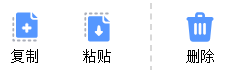
\includegraphics[width=.15\textwidth]{4a.png}
            \task 
\includegraphics[width=.15\textwidth]{4b.png}
            \task 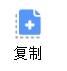
\includegraphics[width=.05\textwidth]{4c.png}
            \task 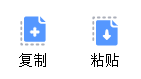
\includegraphics[width=.1\textwidth]{4d.png}
        \end{tasks}

        % 2,4,6 图片
        \begin{figure}[htbp]
            \begin{minipage}[t]{.33\textwidth}
                \centering
                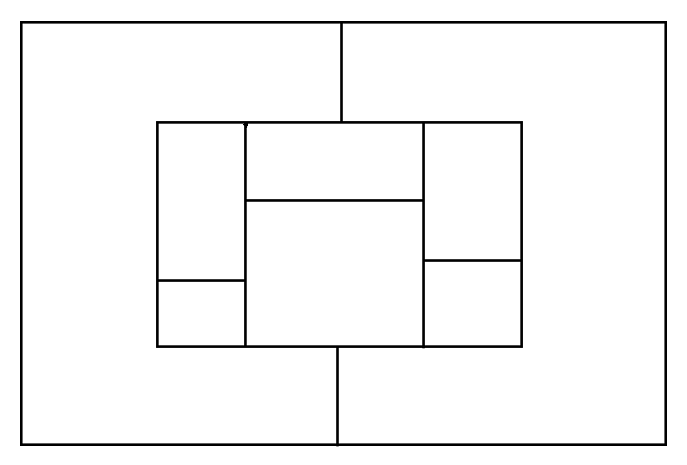
\includegraphics[width=.5\textwidth]{2.png}
                \caption*{第 2 题}
            \end{minipage}
            \begin{minipage}[t]{.33\textwidth}
                \centering
                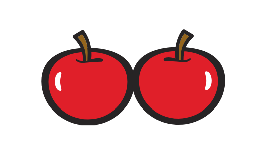
\includegraphics[width=.5\textwidth]{4.png}
                \caption*{第 4 题}
            \end{minipage}
            \begin{minipage}[t]{.33\textwidth}
                \centering
                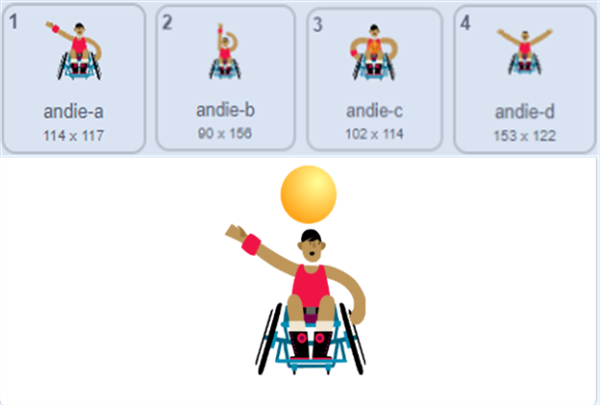
\includegraphics[width=.8\textwidth]{6.png}
                \caption*{第 6 题}
            \end{minipage}
        \end{figure}

        % 5
        \item 完整地播放两次小猫的叫声,以下哪个选项不能实现?(\qquad)
        \begin{tasks}(4)
            \task 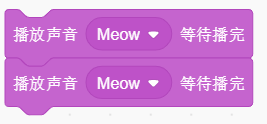
\includegraphics[width=.18\textwidth]{5a.png}
            \task 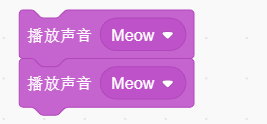
\includegraphics[width=.18\textwidth]{5b.png}
            \task 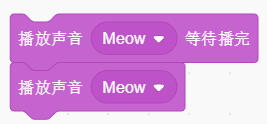
\includegraphics[width=.18\textwidth]{5c.png}
            \task 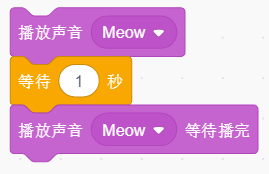
\includegraphics[width=.14\textwidth]{5d.png}
        \end{tasks}

        % 6
        \item 如上图所示,舞台上有 “Andie” 和 “Ball” 两个角色,哪个程序能让角色 “Andie” 的右手碰到黄色的小球?(\qquad)
        \begin{tasks}(4)
            \task 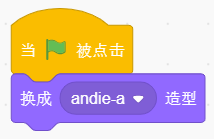
\includegraphics[width=.14\textwidth]{6a.png}
            \task 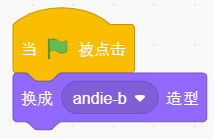
\includegraphics[width=.14\textwidth]{6b.png}
            \task 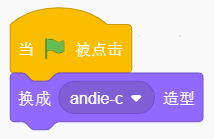
\includegraphics[width=.14\textwidth]{6c.png}
            \task 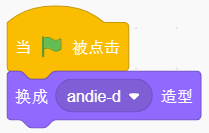
\includegraphics[width=.14\textwidth]{6d.png}
        \end{tasks}

        % 7
        \item 下面哪个积木可以停正正在播放的声音?(\qquad)
        \begin{tasks}(4)
            \task 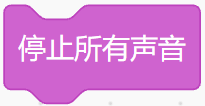
\includegraphics[width=.08\textwidth]{7a.png}
            \task 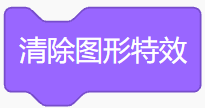
\includegraphics[width=.08\textwidth]{7b.png}
            \task 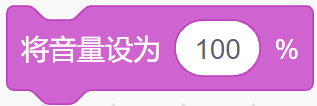
\includegraphics[width=.12\textwidth]{7c.png}
            \task 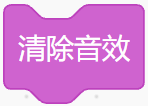
\includegraphics[width=.06\textwidth]{7d.png}
        \end{tasks}

        \newpage
        % 8
        \item 运行下列程序后音调音效为?(\qquad)
        \begin{tasks}(4)
            \task 10
            \task 20
            \task 30
            \task 40
        \end{tasks}

        % 9
        \item 小华、小明和小刘三个人赛跑结束后,小明说:“我跑得不是最快的,但我比小刘跑得快。”他们三人中跑得最快的是?(\qquad)
        \begin{tasks}(4)
            \task 小华
            \task 小明
            \task 小刘
            \task 小唐
        \end{tasks}

        % 10
        \item 默认小猫角色,点击绿旗后,小猫面向什么方向?(\qquad)
        \begin{tasks}(4)
            \task 75
            \task 90
            \task 105
            \task 120
        \end{tasks}

        % 8,10,11,12 图片
        \begin{figure}[htbp]
            \begin{minipage}[t]{.24\textwidth}
                \centering
                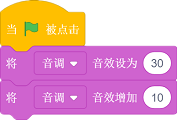
\includegraphics[width=.7\textwidth]{8.png}
                \caption*{第 8 题}
            \end{minipage}
            \begin{minipage}[t]{.24\textwidth}
                \centering
                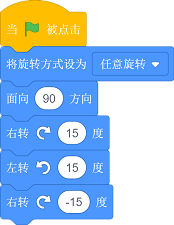
\includegraphics[width=.6\textwidth]{10.png}
                \caption*{第 10 题}
            \end{minipage}
            \begin{minipage}[t]{.24\textwidth}
                \centering
                \begin{minipage}[t]{.45\textwidth}
                    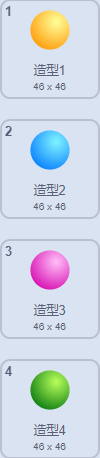
\includegraphics[width=.45\textwidth]{11-1.png}
                \end{minipage}
                \begin{minipage}[t]{.48\textwidth}
                    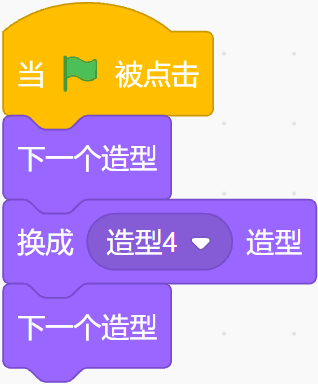
\includegraphics[width=.9\textwidth]{11-2.png}
                \end{minipage}
                \caption*{第 11 题}
            \end{minipage}
            \begin{minipage}[t]{.24\textwidth}
                \centering
                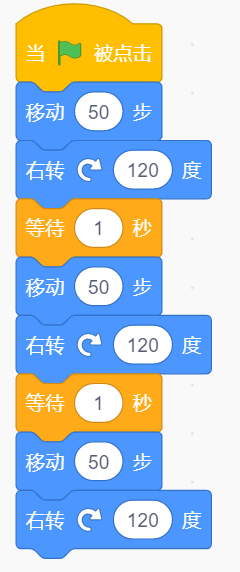
\includegraphics[width=.4\textwidth]{12.png}
                \caption*{第 12 题}
            \end{minipage}
        \end{figure}

        % 11
        \item 执行上图程序,小球的造型为?(\qquad)
        \begin{tasks}(4)
            \task 造型1
            \task 造型2
            \task 造型3
            \task 造型4
        \end{tasks}

        % 12
        \item 小明初始位置在舞台中心,运行上图程序,小明走过的图形是?(\qquad)
        \begin{tasks}(4)
            \task 三角形
            \task 正方形
            \task 长方形
            \task 正五边形
        \end{tasks}

        % 13
        \item 默认小猫角色,执行下列程序,选项正确的是?(\qquad)
        \begin{tasks}(4)
            \task 不旋转
            \task 旋转 50 度
            \task 旋转 90 度
            \task 旋转 140 度
        \end{tasks}

        % 14
        \item 下列哪项操作能把作品保存起来?(\qquad)
        \begin{tasks}(4)
            \task 点击【保存到电脑】
            \task 点击【从电脑中上传】
            \task 点击【新作品】
            \task 点击地球图标
        \end{tasks}

        % 13,14,15,16 图片
        \begin{figure}[htbp]
            \begin{minipage}[t]{.24\textwidth}
                \centering
                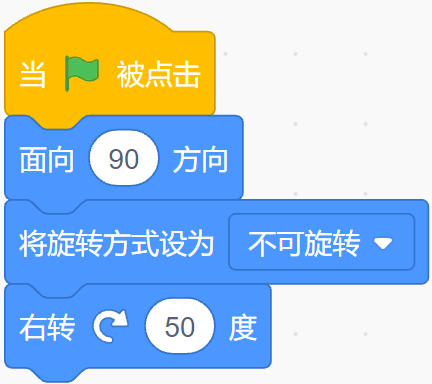
\includegraphics[width=.6\textwidth]{13.png}
                \caption*{第 13 题}
            \end{minipage}
            \begin{minipage}[t]{.24\textwidth}
                \centering
                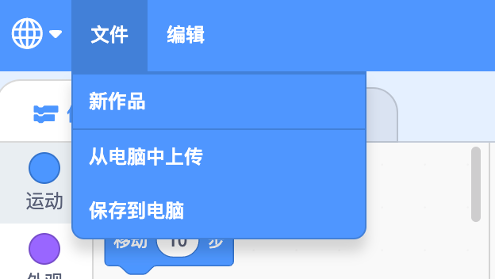
\includegraphics[width=.9\textwidth]{14.png}
                \caption*{第 14 题}
            \end{minipage}
            \begin{minipage}[t]{.2\textwidth}
                \centering
                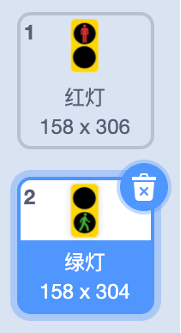
\includegraphics[width=.4\textwidth]{15.png}
                \caption*{第 15 题}
            \end{minipage}
            \begin{minipage}[t]{.3\textwidth}
                \centering
                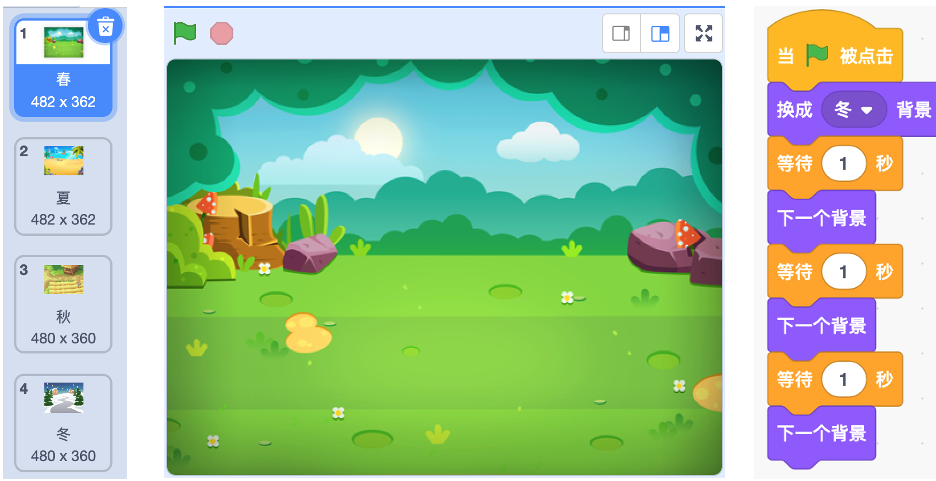
\includegraphics[width=\textwidth]{16.png}
                \caption*{第 16 题}
            \end{minipage}
        \end{figure}

        % 15
        \item 红绿灯角色里有两个造型,当前造型是绿灯,如果想把绿灯切换为红灯,请问下列哪个选项不能实现?(\qquad)
        \begin{tasks}(4)
            \task 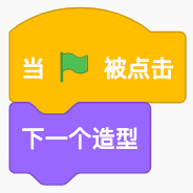
\includegraphics[width=.06\textwidth]{15a.png}
            \task 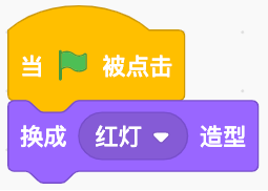
\includegraphics[width=.1\textwidth]{15b.png}
            \task 点击红灯造型
            \task 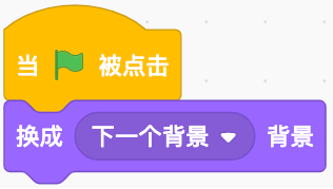
\includegraphics[width=.12\textwidth]{15d.png}
        \end{tasks}

        % 16
        \item 舞台背景和程序如上图所示,程序执行完后,舞台显示的是哪张背景?(\qquad)
        \begin{tasks}(4)
            \task 春
            \task 夏
            \task 秋
            \task 冬
        \end{tasks}

        \newpage
        % 17
        \item 下面关于造型和背景的说法错误的是?(\qquad)
        \begin{tasks}(2)
            \task 角色可以有很多个造型,舞台可以有很多个背景
            \task 可以在角色程序中切换背景
            \task 在舞台程序中,不能切换角色造型
            \task 只能从本地上传角色,不能从本地上传背景
        \end{tasks}

        % 18
        \item 使用下列哪个积木,能够最快捷地让小猫面向老鼠?(\qquad)
        \begin{tasks}(4)
            \task 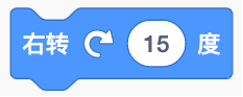
\includegraphics[width=.12\textwidth]{18a.png}
            \task 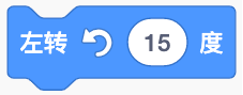
\includegraphics[width=.12\textwidth]{18b.png}
            \task 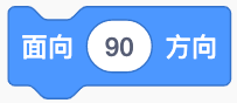
\includegraphics[width=.12\textwidth]{18c.png}
            \task 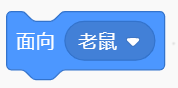
\includegraphics[width=.12\textwidth]{18d.png}
        \end{tasks}

        % 19
        \item 下图是小猴子和香蕉的初始位置,点击一次绿旗,哪个选项的程序可以让小猴子拿到香蕉?(\qquad)
        \begin{tasks}(4)
            \task 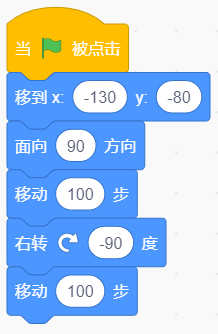
\includegraphics[width=.12\textwidth]{19a.png}
            \task 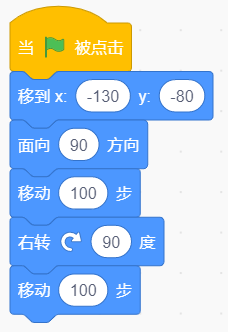
\includegraphics[width=.12\textwidth]{19b.png}
            \task 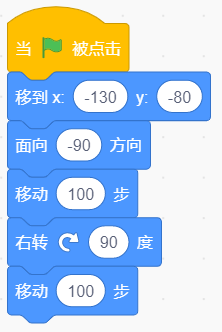
\includegraphics[width=.12\textwidth]{19c.png}
            \task 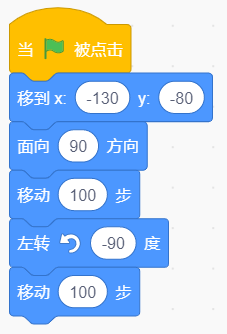
\includegraphics[width=.12\textwidth]{19d.png}
        \end{tasks}

        % 20
        \item 天天制作一个"自我介绍"的作品,他设计的流程是小人先移动100步,然后换成面向观众的造型,最后说:"大家好,我叫天天!",应该把下列程序修改成哪个选项?(\qquad)
        \begin{tasks}(4)
            \task 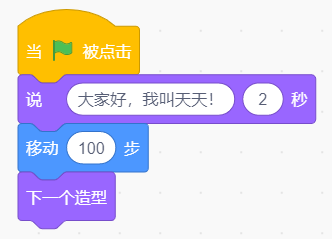
\includegraphics[width=.15\textwidth]{20a.png}
            \task 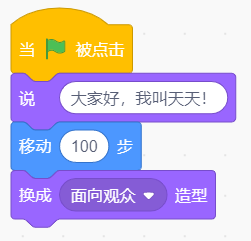
\includegraphics[width=.12\textwidth]{20b.png}
            \task 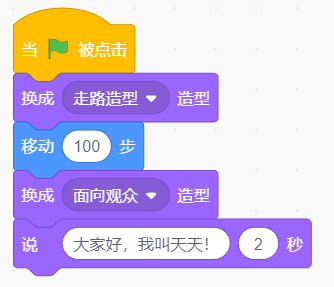
\includegraphics[width=.15\textwidth]{20c.png}
            \task 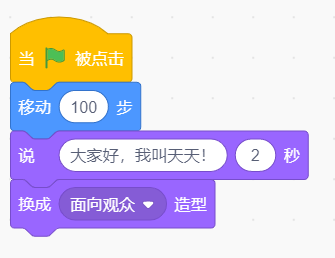
\includegraphics[width=.15\textwidth]{20d.png}
        \end{tasks}

        % 18,19,20,22,23,24 图片
        \begin{figure}[htbp]
            \begin{minipage}[t]{.2\textwidth}
                \centering
                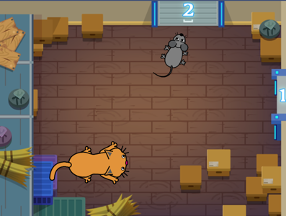
\includegraphics[width=.85\textwidth]{18.png}
                \caption*{第 18 题}
            \end{minipage}
            \begin{minipage}[t]{.2\textwidth}
                \centering
                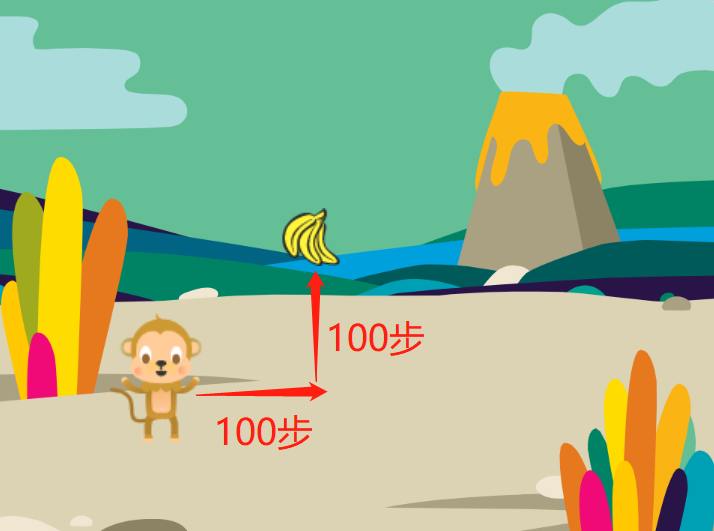
\includegraphics[width=.88\textwidth]{19.png}
                \caption*{第 19 题}
            \end{minipage}
            \begin{minipage}[t]{.24\textwidth}
                \centering
                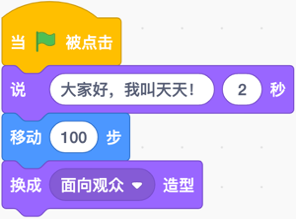
\includegraphics[width=.7\textwidth]{20.png}
                \caption*{第 20 题}
            \end{minipage}
            \begin{minipage}[t]{.1\textwidth}
                \centering
                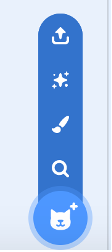
\includegraphics[width=0.6\textwidth]{22.png}
                \caption*{第 22 题}
            \end{minipage}
            \begin{minipage}[t]{.1\textwidth}
                \centering
                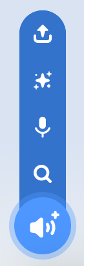
\includegraphics[width=0.45\textwidth]{23.png}
                \caption*{第 23 题}
            \end{minipage}
            \begin{minipage}[t]{.1\textwidth}
                \centering
                
\includegraphics[width=0.45\textwidth]{24.png}
                \caption*{第 24 题}
            \end{minipage}
        \end{figure}

        % 21
        \item 小智做好了一个作品,点击下列哪个按钮可以给全班同学演示这个作品?(\qquad)
        \begin{tasks}(4)
            \task 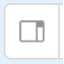
\includegraphics[width=.03\textwidth]{21a.png}
            \task \includegraphics[width=.03\textwidth]{21b.png}
            \task \includegraphics[width=.03\textwidth]{21c.png}
            \task \includegraphics[width=.03\textwidth]{21d.png}
        \end{tasks}

        % 22
        \item 如上图所示,小艾想从角色库里找一个爱心角色,应点击下列哪个按钮?(\qquad)
        \begin{tasks}(4)
            \task \includegraphics[width=.03\textwidth]{22a.png}
            \task \includegraphics[width=.03\textwidth]{22b.png}
            \task \includegraphics[width=.03\textwidth]{22c.png}
            \task \includegraphics[width=.03\textwidth]{22d.png}
        \end{tasks}

        % 23
        \item 如上图所示,下列哪个选项可以给角色录制声音?(\qquad)
        \begin{tasks}(4)
            \task \includegraphics[width=.03\textwidth]{23a.png}
            \task \includegraphics[width=.03\textwidth]{23b.png}
            \task \includegraphics[width=.03\textwidth]{23c.png}
            \task \includegraphics[width=.03\textwidth]{23d.png}
        \end{tasks}

        % 24
        \item 如上图所示,小明想导入一个素材库中没有的背景,应点击下列哪个图标?(\qquad)
        \begin{tasks}(4)
            \task \includegraphics[width=.03\textwidth]{24a.png}
            \task \includegraphics[width=.03\textwidth]{24b.png}
            \task \includegraphics[width=.03\textwidth]{24c.png}
            \task \includegraphics[width=.03\textwidth]{24d.png}
        \end{tasks}

        % 25
        \item 舞台背景没有下列哪一类积木?(\qquad)
        \begin{tasks}(4)
            \task 外观类
            \task 事件类
            \task 运动类
            \task 控制类
        \end{tasks}
    \end{enumerate}

    % 判断题
    \newpage
    {\noindent\textbf{第二部分、判断题(共 10 题,每题 2 分,共20分.)}}
    \begin{enumerate}
        \setcounter{enumi}{25}
        % 26
        \item 从角色库选择的角色,如果是位图模式,不能改为失量图模式。(\qquad)

        % 27
        \item 可以在舞台背景图片中添加英文,但文字的大小和颜色是不能修改的。(\qquad)

        % 28
        \item 运行下列程序,"同学们大家好!"与"我们一起来学编程吧。"这两句话是同时出现2秒。(\qquad)

        % 29
        \item 不能给舞台背景选择声音,并播放出来。(\qquad)

        % 8,10,11,12 图片
        \begin{figure}[htbp]
            \begin{minipage}[t]{.24\textwidth}
                \centering
                \includegraphics[width=\textwidth]{28.png}
                \caption*{第 28 题}
            \end{minipage}
            \begin{minipage}[t]{.24\textwidth}
                \centering
                \includegraphics[width=.3\textwidth]{33.png}
                \caption*{第 33 题}
            \end{minipage}
            \begin{minipage}[t]{.24\textwidth}
                \centering
                \begin{minipage}[t]{.38\textwidth}
                    \includegraphics[width=.8\textwidth]{34-1.png}
                \end{minipage}
                \begin{minipage}[t]{.58\textwidth}
                    \includegraphics[width=\textwidth]{34-2.png}
                \end{minipage}
                \caption*{第 34 题}
            \end{minipage}
        \end{figure}

        % 30
        \item 有四个箱子,蓝箱子比黄箱子大,蓝箱子比黑箱子小,黑箱子比红箱子小,四个箱子中最大的是蓝箱子。(\qquad)

        % 31
        \item 双击一段程序的第一个积木,可以来执行这段程序。(\qquad)

        % 32
        \item 小猫有两个造型,当前造型是第二个造型,执行下列积木\includegraphics[width=.07\textwidth]{32.png},小猫将变成第一个造型。(\qquad)

        % 33
        \item 默认小猫角色程序如上图所示,点击绿旗后,并没有看到小猫移动和旋转。(\qquad)
        
        % 34
        \item 上图程序可以完整地播完三个声音(\qquad)

        % 35
        \item 复制角色时,只能复制角色的造型和声音,不能复制程序。(\qquad)
    \end{enumerate}

    \newpage
    {\noindent \textbf{第三部分、编程题(共 2 题,共30分.)}}
    \begin{enumerate}
        \setcounter{enumi}{35}
        
        % 36
        \item 章鱼表演:
        
        1. 准备工作
        \begin{tasks}[label = (\arabic*)]
            \task 选择背景:Underwater1, Underwater2;
            \task 选择角色:Octopus;
            \task 选择背景声音:Bossa Nova。
        \end{tasks}
        2. 功能实现
        \begin{tasks}[label = (\arabic*)]
            \task 点击开始,角色 Octopus 初始位置在舞台左侧中部,初始造型为 Octopus-b,初始背景为 Underwater1;
            \task 角色 Octopus 从舞台左侧移动到右侧,不断改变造型;
            \task 章鱼到达舞台最右边后,切换为 Underwater2,章鱼移到舞台中心位置;
            \task 背景播放 Bossa Nova 声音。
        \end{tasks}
        \begin{figure}[htbp]
            \centering
            \includegraphics[width=.26\textwidth]{36.png}
        \end{figure}

        %37
        \item 小猫飞翔:
        
        1. 准备工作
        \begin{tasks}[label = (\arabic*)]
            \task 保留小猫角色,删除造型 cat-b,添加 Cat Flying-a 造型;
            \task 添加 Blue Sky 和 Blue Sky2 背景,删除背景1,把小猫移到舞台左下角。
        \end{tasks}
        2. 功能实现
        \begin{tasks}[label = (\arabic*)]
            \task 初始背景为 Blue Sky,小猫造型为 cat-a,面向右;
            \task 点击小猫以后,小猫说:"起飞!" 2 秒;
            \task 小猫说完以后,换成 Cat Flying-a 造型,1 秒以后面向 45 度方向;
            \task 接下来每隔 1 秒移动 100 步,移动 3 次以后,背景换成 Blue Sky2。
        \end{tasks}

        \begin{figure}[htb]
            \centering
            \begin{minipage}[t]{.19\textwidth}
                \centering
                \includegraphics[width=.9\textwidth]{37-2.png}
            \end{minipage}
            \begin{minipage}[t]{.19\textwidth}
                \centering
                \includegraphics[width=.9\textwidth]{37-3.png}
            \end{minipage}
            \begin{minipage}[t]{.19\textwidth}
                \centering
                \includegraphics[width=.9\textwidth]{37-4.png}
            \end{minipage}
            \begin{minipage}[t]{.19\textwidth}
                \centering
                \includegraphics[width=.9\textwidth]{37-5.png}
            \end{minipage}
            \begin{minipage}[t]{.19\textwidth}
                \centering
                \includegraphics[width=.9\textwidth]{37-1.png}
            \end{minipage}
        \end{figure}
    \end{enumerate}
\end{document}